\begin{figure}[htbp]
\section*{ ITPR1}
\centering
\begin{subfigure}[b]{0.95\textwidth}
\centering
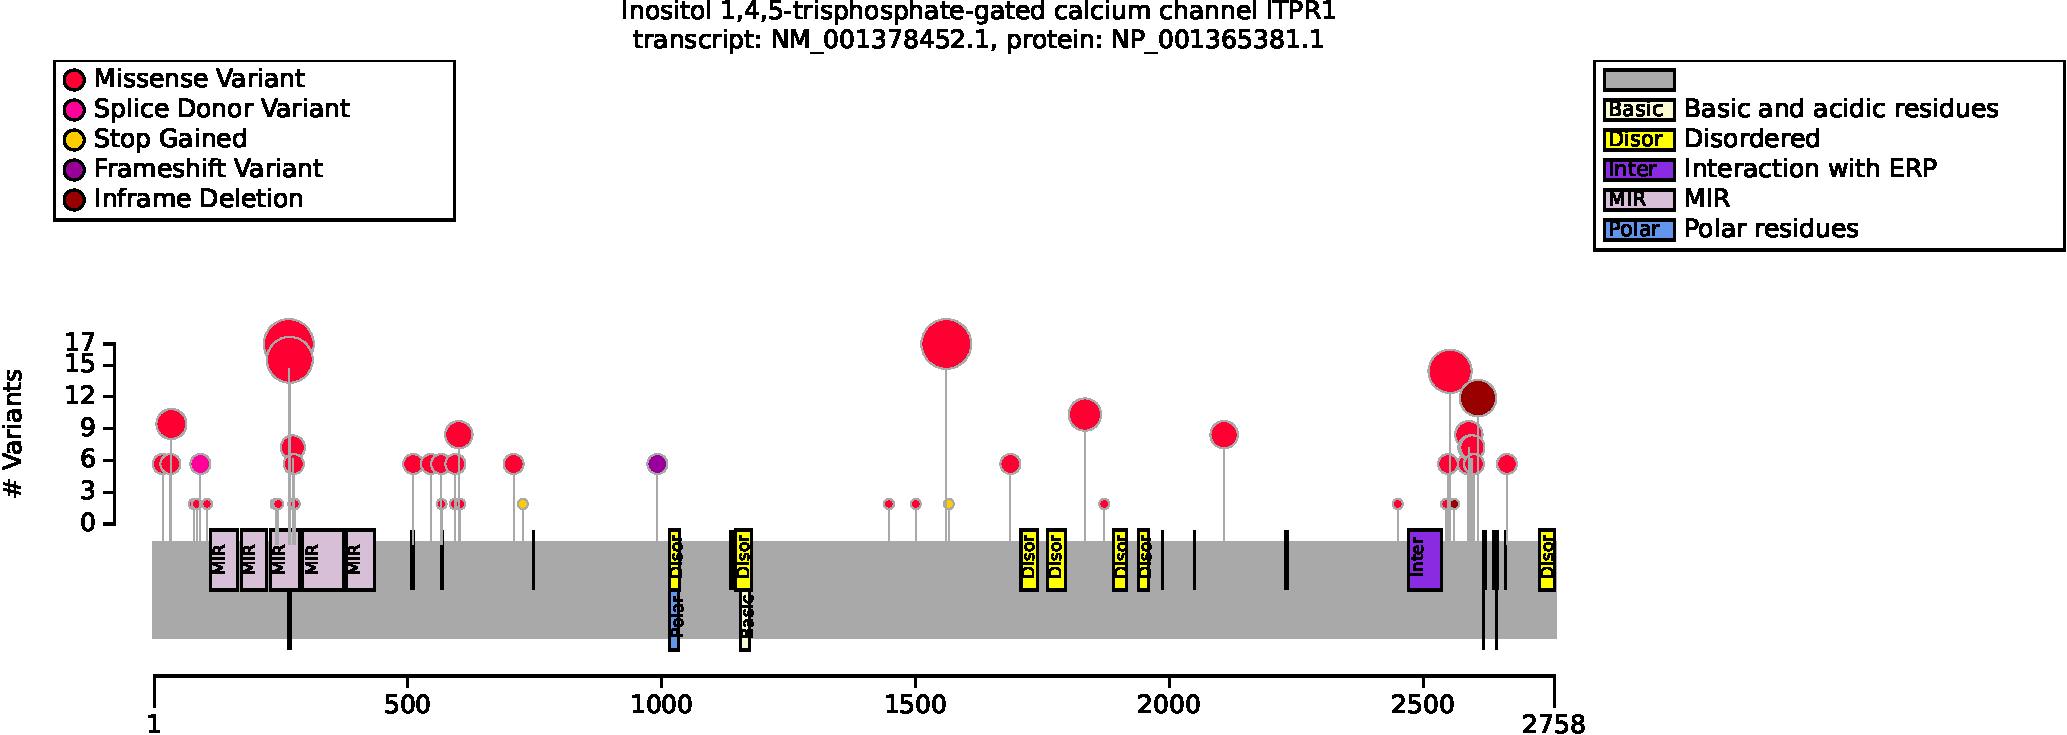
\includegraphics[width=\textwidth]{ img/ITPR1_protein_diagram.pdf} 
\captionsetup{justification=raggedright,singlelinecheck=false}
\caption{Distribution of variants in ITPR1}
\end{subfigure}

\vspace{0.2em}

\begin{subfigure}[b]{0.95\textwidth}
\centering
\resizebox{\textwidth}{!}{
\begin{tabular}{llllrr}
\toprule
HPO term & IP3 binding & other & p-value & adj. p-value\\
\midrule
Delayed speech and language development [HP:0000750] & 13/13 (100\%) & 37/63 (59\%) & 0.003 & 0.019\\
Neurodevelopmental delay [HP:0012758] & 29/29 (100\%) & 70/90 (78\%) & 0.003 & 0.019\\
Aniridia [HP:0000526] & 0/14 (0\%) & 20/54 (37\%) & 0.007 & 0.024\\
Delayed gross motor development [HP:0002194] & 18/18 (100\%) & 57/83 (69\%) & 0.005 & 0.024\\
Motor delay [HP:0001270] & 24/24 (100\%) & 63/89 (71\%) & 0.002 & 0.019\\
Nystagmus [HP:0000639] & 25/26 (96\%) & 53/78 (68\%) & 0.003 & 0.019\\
Delayed ability to sit [HP:0025336] & 11/11 (100\%) & 42/70 (60\%) & 0.013 & 0.043\\
Delayed ability to walk [HP:0031936] & 13/13 (100\%) & 41/68 (60\%) & 0.004 & 0.019\\
\bottomrule
\end{tabular}
}
\captionsetup{justification=raggedright,singlelinecheck=false}
\caption{Fisher Exact Test performed to compare HPO annotation frequency with respect to IP3 binding and other. Total of 26 tests were performed.}
\end{subfigure}
\vspace{0.2em}
\begin{subfigure}[b]{0.95\textwidth}
\centering
\resizebox{\textwidth}{!}{
\begin{tabular}{llllrr}
\toprule
HPO term & SV Deletion & other & p-value & adj. p-value\\
\midrule
Delayed speech and language development [HP:0000750] & 0/19 (0\%) & 50/57 (88\%) & $1.72\times 10^{-12}$ & $7.57\times 10^{-12}$\\
Neurodevelopmental delay [HP:0012758] & 0/19 (0\%) & 99/100 (99\%) & $4.07\times 10^{-21}$ & $8.96\times 10^{-20}$\\
Delayed gross motor development [HP:0002194] & 0/19 (0\%) & 75/82 (91\%) & $4.04\times 10^{-15}$ & $2.96\times 10^{-14}$\\
Motor delay [HP:0001270] & 0/19 (0\%) & 87/94 (93\%) & $3.90\times 10^{-16}$ & $4.29\times 10^{-15}$\\
Global developmental delay [HP:0001263] & 0/19 (0\%) & 48/57 (84\%) & $1.81\times 10^{-11}$ & $5.68\times 10^{-11}$\\
Nystagmus [HP:0000639] & 17/17 (100\%) & 61/87 (70\%) & 0.006 & 0.016\\
Delayed ability to sit [HP:0025336] & 0/19 (0\%) & 53/62 (85\%) & $4.56\times 10^{-12}$ & $1.67\times 10^{-11}$\\
Delayed ability to walk [HP:0031936] & 0/19 (0\%) & 54/62 (87\%) & $1.47\times 10^{-12}$ & $7.57\times 10^{-12}$\\
\bottomrule
\end{tabular}
}
\captionsetup{justification=raggedright,singlelinecheck=false}
\caption{Fisher Exact Test performed to compare HPO annotation frequency with respect to SV Deletion and other. Total of 22 tests were performed.}
\end{subfigure}
\end{figure}

% Next page

\begin{figure}[htbp]\ContinuedFloat
\begin{subfigure}[b]{0.95\textwidth}
\centering
\resizebox{\textwidth}{!}{
\begin{tabular}{llllrr}
\toprule
HPO term & GS Hotspot & other & p-value & adj. p-value\\
\midrule
Aniridia [HP:0000526] & 14/20 (70\%) & 6/48 (12\%) & $6.13\times 10^{-6}$ & $1.59\times 10^{-4}$\\
Delayed gross motor development [HP:0002194] & 18/18 (100\%) & 57/83 (69\%) & 0.005 & 0.032\\
Motor delay [HP:0001270] & 19/19 (100\%) & 68/94 (72\%) & 0.006 & 0.032\\
Delayed ability to sit [HP:0025336] & 13/13 (100\%) & 40/68 (59\%) & 0.003 & 0.030\\
Delayed ability to walk [HP:0031936] & 14/14 (100\%) & 40/67 (60\%) & 0.003 & 0.030\\
\bottomrule
\end{tabular}
}
\captionsetup{justification=raggedright,singlelinecheck=false}
\caption{Fisher Exact Test performed to compare HPO annotation frequency with respect to GS Hotspot and other. Total of
        25 tests were performed. }
\end{subfigure}

\vspace{0.2em}

\caption{The cohort comprised 170 individuals (65 females, 41 males, 64 with unknown sex). 1 of these individuals was reported to be deceased. 
A Fisher exact test for male/female differences revealed no significant associations.
A total of 196 HPO terms were used to annotate the cohort. Disease diagnoses: Spinocerebellar ataxia 29, congenital nonprogressive (OMIM:117360) (104 individuals), Gillespie syndrome (OMIM:206700) (39 individuals), Spinocerebellar ataxia 15 (OMIM:606658) (27 individuals). A total of 62 unique variant alleles were found in \textit{ITPR1} (transcript: \texttt{NM\_001378452.1}, protein id: \texttt{NP\_001365381.1}).}
\end{figure}
